\documentclass[12pt]{article}                           % Document class -- add [12pt] before {article} for 12pt font
\usepackage[letterpaper, margin=1in]{geometry}    % Paper type and margin size
\usepackage[english]{isodate}                     % Sets the date to US style
\usepackage[USenglish]{babel}                     % US English as language
\usepackage[utf8]{inputenc}                       %
\usepackage{amsmath,amsthm,amssymb,amsfonts}      % Math packages
\usepackage[margin=10pt,font=small,labelfont=bf, labelsep=endash]{caption}
\usepackage{longtable}                            % Package for longtables
\usepackage{lscape}                               % Landscape tables
\usepackage{epigraph}                             % Pretty quotes with \epigraph{}
\usepackage{booktabs,calc}
\usepackage{tikz}
\usetikzlibrary{decorations.text,calc,arrows.meta}
\usepackage{graphicx}                             % Allows the import of graphs and figures
\graphicspath{ {images/} }
\usepackage{caption}
\usepackage{subcaption}
\usepackage{pdflscape}
% \pagestyle{empty}
% \usepackage[activate={true,nocompatibility},final,tracking=true,kerning=true,spacing=true,factor=1100,stretch=10,shrink=10]{microtype}
\usepackage{lastpage}                             % For page number in footer
\usepackage{todonotes}                            % To do list in the text
\usepackage{multicol}                             % Multiple columns
\usepackage{natbib}                               % Bibliography package
\setcitestyle{aysep={}}                           % Author Year (no comma)
\usepackage{parskip}                              % No default indent
\usepackage{setspace}                             % Adjust line-spacing
\usepackage{mathptmx}      %this package and the one below it allow Times New Roman font usage
\usepackage[T1]{fontenc}
\usepackage{endnotes}      %convert footnotes to endnotes
\let\footnote=\endnote
%\singlespacing
% \onehalfspacing
\doublespacing
\usepackage{rotating}                             % Rotate figures and tables
\usepackage{bm}                                  % Use Greek boldface \bm{\beta}
% \microtypecontext{spacing=nonfrench}
\usepackage{float}


\begin{document}

\title{Gift Travel in the U.S. House of Representatives}
\author{Anonymous}
\date{\today}



\maketitle

\thispagestyle{empty}

\newpage
\abstract{Fear of interest group influence on the American political system remains an exceptionally prevalent concern in the American mind. Scholars have long sought to shed light on the ways in which this influence might manifest itself. One significantly understudied avenue is that of privately sponsored travel by members of Congress. Previous work studying this so-called gift travel has relied on data collected by a private watchdog organization. This paper presents new data provided by members to the Clerk of the House from 2007 to 2019. Members of the House of Representatives (and their staff) reported taking 10,364 trips during that time, with each member traveling an average of 4.75 times per congress. We seek to explain the variation in this travel and update the scholarly understanding of this increasingly prevalent practice. We find that members are taking more privately sponsored trips than ever regardless of how long they have served in Congress. Moreover, previous findings of decreased travel when a member faced a close election no longer holds true. Interest groups, think tanks, and other private organizations are targeting members with institutional power and those who are more ideologically extreme. Our findings suggest a weakening fear of retribution for privately sponsored travel among members of Congress possibly tied to the extensive polarization that has occurred since the last study of gift travel.}
\begin{center} Key Words: gift travel; privately sponsored travel; Congress; congressional delegations; congressional travel; \end{center}
\thispagestyle{empty}

\newpage
\setcounter{page}{1}
\pagenumbering{arabic}

Gift travel occurs when a member, or one of her staff, goes on an expense-paid trip sponsored by a non-governmental organization, such as a trade association, think tank, cable channel, or university. Going on an expense-paid trip, because it involves an investment of time and attention, can be extremely meaningful for a relationship between a member and an interest group. Time, as scholars know, may be a legislator's most important resource \citep[34]{Fenno1978}. In compliance with House ethics rules, when members go on these sponsored trips, they must report them to the Clerk of the House.\footnote{According to Rule XXV, clause 5 of the Rules of the House of Representatives, members must disclose reimbursement for such travel within 15 days of return. The Clerk of the House makes a report of these disclosures public on its website.} These reporting rules, as \cite{Rosenson2009} suggests, are likely in response to perceptions of corruption among the public. Since these reporting requirements have gone into place members reported spending 42,388 days on 10,364 gift trips over the 2007-2019 period, with each member traveling an average 19 days per congress. Who is paying for this travel and why? Which members are selected to go on trips? What do these trips mean for governance? These questions are critical to our understanding of privately sponsored travel and to Congress as an institution more generally.

%Our argument is built upon the scholarship that has failed to find a link between campaign contributions and roll-call votes \citep{Welch1982,Wright1990}. Moreover, we seek to build upon scholarship that has argued for a more nuanced relationship between interest groups and members, like contributions timed before key votes or committee markups \citep{Stratmann1998,Hall1990}, contributions in exchange for meetings with members \citep{Langbein1986}, and the provision of information or services to members' offices \citep{Hall2006}.
%This nuanced approach to interest group and member behavior is consistent with previous research on privately sponsored travel. \cite{Rosenson2009} argues that trip sponsors may have multiple goals in sending members on trips and that members have various reasons for accepting their invitations. She finds that institutional power, ideology, and seniority all play a role in predicting trips by members or their staffs \citep{Rosenson2009}. We examine a broader period of activity than Rosenson, though only for House members, and utilize data reported directly to the Clerk of the House instead of to a third party.
%We present three major findings. First, party leaders, committee chairs, and ranking members travel much more than the rank and file, which is consistent with Rosenson's data from 2001-2004. Second, seniority is not a significant predictor of the number of gift travel trips a member goes on, and electoral safety has only a trivial effect. Third, and unexpectedly, more ideologically extreme members travel more than their moderate colleagues.

Despite a lack of scholarly attention, gift travel has already been highlighted by the popular media as potentially corruptive. For example, at the end of May 2013, ten members of Congress, along with thirty-two staffers and dozens of state legislators, traveled to Baku, Azerbaijan. Gathering on the shore of the Caspian Sea, they took part in an all-expense-paid conference and cultural visit. The members and their staff listened to speeches given by the president of Azerbaijan, three former advisers to President Obama, and attended at least three briefings pertaining to the country's state-owned oil company. The trip sparked controversy when it was reported that the Azerbaijan-affiliated nonprofits that sponsored the travel had used money originating from a state agent, the very same state-owned oil company that had held information sessions during the conference \citep{Tucker2014}.

While it is legal for nongovernmental organizations to pay for members to go on such excursions, members are forbidden from accepting travel offers from foreign countries or corporations that employ U.S. lobbyists, and members may not meet with lobbyists at any time during their travel \citep{Wickham2015}. The Baku trip highlights the potential for gift travel to be gamed by the sponsors, the laxness of the self-reporting system, and the difficulty in connecting what goes on during these trips with legislators' preferences and behavior. While this particular trip was unusual because it may have involved breaking federal law, in many other ways it was an ordinary instance of gift travel. Members were invited by a nonprofit to listen to speeches in and tour around a foreign country. The speeches, briefings, and mingling were all a part of what a member typically experiences on a gift-travel trip.

Previous work on privately sponsored travel utilized data collected by a private watchdog organization and those data are now over a decade old \citep{Rosenson2009}. This paper seeks to explain the variation in this gift travel and update the scholarly understanding of it using the data members' offices are now required to disclose. Rosenson tests a large number of variables, uncovering many interesting results such as increased travel due to positions of institutional power, seniority, membership on the Foreign Affairs Committees and even a member's race. She also finds that decreases in travel occur for members on prominent power committees, retiring members, and members who are electorally vulnerable. A subset of her variables yield neutral or inconclusive results such as the role of constituent preferences, being a subcommittee chair, or being in the majority party. While we do not test each of these variables in this paper, we have identified the variables we believe to be most crucial to explaining member travel since Rosenson's work.

While money is generally seen as the most important resource to many politicos, we argue that the scarcity of time on Capitol Hill is of far greater importance due to its scarcity. Any time spent on gifted trips during recess is time not spent in the district and, any time spent while the House is in session needs to be coordinated with leadership to ensure no important votes will be missed.\footnote{Note that occasionally gifted trips occur with state delegations, which may entail members visiting their own districts. Most trips occur outside of members' districts.} Though it is often the case that members' staff take these trips rather than the members themselves, with only a limited number of staff, such trips also use up the offices' precious time.  Put simply, gift travel requires much more activity from a member than simply receiving a check.

We theorize that organizations sponsor trips in pursuit of information exchange, the opportunity to have the member's attention, and the opportunity to build a long-term relationship. Therefore, we conjecture that groups target members who are strategically positioned to influence the legislative process. Such members will likely be among the party leadership \citep{Cox2005,Rosenson2009}, electorally safe \citep{Grimmer2013a}, senior \citep{Rosenson2009,Snyder1992}, and relatively moderate ideologically \citep{Alduncin2017}. Sponsors are typically specialized organizations, like trade associations or think tanks, and must balance their preferences for power, policy specialization, and the probability of influence \citep{Hall2006}. While every group might want to get the ear of the Speaker of the House, only the most resourceful sponsors are apt to do so. Others must take what they can get, and use their finances wisely \citep{Barber2017}.

We find that gift travel is occurring more every year, further underscoring the need for renewed scholarly attention to it. We validate Rosenson's finding that members with institutional power tend to go on more trips, and especially if they are ideologically extreme. But, we identify two key differences from Rosenson's work as well. First, seniority no longer seems to increase the number of trips a member takes. This finding is likely attributable to the degradation of the seniority system for accumulating power within Congress that began in the 1990s and has only increased since Rosenson's data were collected \citep{Sinclair2012,Theriault2008}. Second, the fear of going on too many privately funded trips if a member was facing reelection or expecting to be in a close race has dissipated. This finding is particularly concerning for governance and accountability within Congress. Moreover, it mirrors the problem expressed by money-in-politics scholars studying other avenues of influence by private actors. That is, campaign contributions (or gift travel) might be feverishly documented and published online, but accountability by constituents is often lacking, and this transparency can even lead to decreased trust in government \citep{Primo2006}. Taken together these findings represent a renewed look at privately sponsored member travel and can direct future work with these data. We will now turn to the data and detail what we know about gift travel. We close the paper with a more detailed discussion of our findings, their implications, and suggestions for avenues of future research on gift travel and member behavior in Congress.

\subsection*{\centering Data}

Every year since 2007, the Office of the Clerk of the U.S. House of Representatives has published all gift travel reports. This paper analyzes these reports from the 110th through the 115th Congresses (2007-2019). These data, after cleaning, collapsing duplicate trip entries, and aggregating by member, consist of 2,619 observations, which are at the level of the member per congress. Over the course of the eleven-year period for which we have data, each member, or their staff, traveled an average 19 days per congress and reported spending a total of 42,388 days (on 10,364 trips) engaged in gift travel; the average trip is about four days.

[Figure 1 about here]

Despite the sawtooth pattern, indicating that members tend to take more trips in the first session of a Congress than the second, there is a clear trend of increasing trips over time (vertical lines separate congresses). While members only took about 300 trips in 2007, they quickly were taking over 1000 trips per year by 2011 and peaked over 1500 trips per year in 2017. This trend alone should be enough to underscore the importance of explaining variation in privately-sponsored travel and continued vigilance by both scholars and the public alike.

After attempting to correct for typos and various names for the same organization, we found that a total of 1,466 nongovernmental sources provided reimbursement for travel to members of Congress between 2007 and 2019.\footnote{Filing these reports is left up to the members and their staffs. It is up to them to spell the name of the sponsor correctly, use the full name or an abbreviation, and, indeed, know exactly who it is that is sponsoring the trip. Because of this, the true number of sponsors is likely slightly lower than 1,466.} Each of these organizations gave at least one gift-trip in that eleven-year period, which equates to about 250 organizations per Congress, with each congressional cohort taking about 2,500 trips.

A small number of familiar names are responsible for a hefty portion of the number of trips taken each congress. Only about 4\% (63 out of 1466) of the sponsoring organizations averaged at least one trip per Congress, or five total in the data set. This datum would imply that only five or six dozen organizations are assuming the cost of putting members on trips as a regular part of business. The other 95\% or so appear to be using gift travel only sparingly, possibly in reaction to shifts in the policy agenda or opportunities to alter the policy content of bills \citep{Hall1990}. The sixty-two organizations that, on average, sponsored one or more trips per Congress account for 72\% of the all the reported trips in our data set. The concentration of gifting behavior among a handful of sponsors is an important descriptive fact to note. See Appendix Table A1 for a list of the top travel sponsors.

To get some notion of who the big players are, let's look briefly at the top five sponsors. The most active sponsor, by far, is an organization called the Congressional Institute, which provided travel subsidies an average of 392 occasions per Congress. The Congressional Institute appears to invite great numbers of members, usually around 150 of them, to places near Washington, such as Hot Springs, Virginia. This is the same group that \cite{Rosenson2009} indicated as the top sponsor. The remaining travel sponsors are the American Israel Education Foundation (146 trips per Congress), the Aspen Institute (116), the Heritage Foundation (92), and the United Nations Foundation (78). The Aspen Institute and the Heritage Foundation are think tanks; the United Nations Foundation is an international NGO seeking to build support for the UN and its activities; and the American Israel Education Foundation is an interest group, self-described as being part of America's pro-Israel lobby.

[Table 1 about here]

Of the top 25 groups in Rosenson's study only six groups overlap.\footnote{Our data are restricted to trips sponsored for House members whereas Rosenson examined both House and Senate trips.} Those groups are the Congressional Institute, the Aspen Institute, the American Israel Education Foundation, the Heritage Foundation, the Consumer Electronics Association and the Congressional Black Caucus; each group is higher on our list than were on Rosenson's. Notably, many of the groups are different but still evoke similar ideological or policy-area specific concerns. The biggest difference is an increased presence of universities on the list.

The dependent variable for our analysis is \emph{trips}. It is a count, i.e., a sum of binary items (traveled or did not), and it is over-dispersed.\footnote{Overdispersion occurs when the observed variance is larger than the expected variance from a given model. The count is the number of separate journeys reported by each member to the Clerk of the House; each unique report counts as one trip.} Further, there is heterogeneity across individuals' probabilities of traveling. We estimate a negative binomial regression using maximum likelihood, and include fixed-effects for each Congress. The full regression results can be found in the Appendix Table A1.

Our trips variable is aggregated at the office level. Members do not go on every trip themselves. We argue this aggregation is appropriate because a member's office is instrumental to her legislative behavior \citep{Mayhew1974}, and because sponsors continue to provide travel even though staffers are the ones visiting. The data indicate that members go on only about 30\% of the trips they report; the remaining 70\% are attended by staffers. In fact, the proportion of trips taken by staffers, when broken down by Congress, shows that members are attending fewer and fewer trips each congressional biennium. And, even though members are attending smaller proportions of trips each year, the total number of trips reported each year continues to grow.

Not all members (or their staffers) go on gift travel, but most of them do. Of the 2,180 total members, 292 (13.4\%) did not go on a single trip. Similarly, 253 members (11.6\%) went on exactly one, 42 (11.4\%) went on two, 255 (11.7\%) went on three, with 4.8 trips being the mean. Figure A1 shows a histogram of the number of trips taken by all the members. The figure is heavily right-skewed (mean = 4.8, sd = 4.7, median = 4), with only 30 members total (or 6 per Congress) going on 20 or more trips.

Democrats travel less often, on average, compared to Republicans (see Figure A2). The average number of trips among Democrats is 4.3, but the variance is large ($\sigma^2 = 23.7$). Republicans, on average, go on one more trip than Democrats; their average is 5.2, but again, the variance is large ($\sigma^2 = 20.3$). This finding is contrary to Rosenson's finding that Democrats tend to travel more during her sample period of 2001-2004.

Of course, not all trips are the same. Some trips involve foreign travel, while others entail just a quick jaunt into a state bordering the District of Columbia. Twenty-nine percent of all trips, on average, involved travel outside the United States. Figure A4 shows that, with the exception of the 114th Congress, foreign trips are growing in number, as are domestic trips. As suspected, members have a clear preference for taking foreign trips instead of sending their staffers in their place (see Figures A6 and A7). And, their preference has grown stronger over time. Members in the 113th and 114th Congresses attended about half of the foreign trips compared to one-third of foreign trips in the 110th Congress. Conversely, in the 110th, members went on 37\% of all domestic trips; by the 114th, that number had shrunk to 14\%. Over time, offices are going on more total trips, but the members are sending their staffers to many of the domestic destinations.

\subsection*{\centering Results and Discussion}

What characteristics separate those who travel often from those who stay in Washington or only travel to their districts? The predicted counts reported in Table 2 offer answers to this question.\footnote{See Appendix Table A2 for the full regression results.} The statistically significant parameter estimates for these position-of-power variables---party leaders, committee chairs, and ranking members---indicate that powerful members travel more, but the coefficients alone do not give us a clear idea of how many more trips per Congress they go on. For the substantive meaning of the regression estimates, we calculate predicted number of trips. Holding all other power variables at zero and the continuous variables, \emph{seniority}, \emph{win percentage}, and \emph{ideological extremity}, at their sample means, the effect of being party leader is sizable: a party leader is predicted to go on 5.49 trips per Congress, three more trips than a rank-and-file member, an increase of 113\% (see Table 2). The effect of being a committee chair is almost identical in size to that of being a party leader, while the effect of ranking member differs across party.

[Table 2 about here]

The interactive effect of ideological extremity and party on the number of gift-travel trips members go on is a significant finding of this paper. It is important not only because the magnitude of its effect is large but also because it reveals how ideology works to attract sponsors toward members in different degrees depending on their party. The large positive effect of ideological extremity holds for members of both parties, but the size of the effect is larger for Democrats than it is for Republicans. Visualized in Figure 2, the predicted number of trips for Republicans can be seen to rise from 2.1 to 3.3 (57\% increase), while the number for Democrats jumps from 0.9 to 4.8 (433\% increase). So, what a Democrat may lack in committee power in the eyes of sponsors, she may make up for if her views are sufficiently liberal.

[Figure 2 about here]

We also find some interesting null effects and observe two noteworthy trends. First, though we expected otherwise, more senior and electorally safe members are no more likely than their marginal freshman counterparts to take a trip on someone else's dime. Second, since gift travel has been reported in its current fashion, members have only gone on more and more trips per congressional term. The findings uncovered in this paper underscore the changing nature of privately-sponsored travel by members of Congress. The decay of internal norms (e.g. the seniority system) and the increase of partisan polarization in Congress have served to decreased accountability related to gift travel despite increased transparency of the practice. And, as the prevalence of taking privately-sponsored trips only seems to increase over time it is clear that more work needs to be done to sort out what effects these trips might have on policymaking. Future work should address such concerns as well as dig deeper into questions already tackled within the literature on Congressional delegations such as who travels with whom and how often \citep{Alduncin2014,Alduncin2017}. Much work remains to be done in this area and the aggregation of this new and publicly available data provide an ideal opportunity to continue digging.

\newpage
\theendnotes

\newpage
\begin{thebibliography}{xx}

\harvarditem[Alduncin, Parker \harvardand\ Theriault]{Alduncin, Parker
  \harvardand\ Theriault}{2017}{Alduncin2017}
Alduncin, Alexander, David C.~W. Parker \harvardand\ Sean~M. Theriault. 2017.
\newblock ``Leaving on a {{Jet Plane}}: {{Polarization}}, {{Foreign Travel}},
  and {{Comity}} in {{Congress}}.'' {\em Congress \& the Presidency} pp.~1-24.

\harvarditem[Alduncin et~al.]{Alduncin, Kelly, Parker \harvardand\
  Theriault}{2014}{Alduncin2014}
Alduncin, Alexander, Sean~Q. Kelly, David C.~W. Parker \harvardand\ Sean~M.
  Theriault. 2014.
\newblock ``Foreign {{Junkets}} or {{Learning}} to {{Legislate}}?
  {{Generational Changes}} in the {{International Travel Patterns}} of {{House
  Members}}, 1977-2012.'' {\em The Forum} 12(3).

\harvarditem[Barber, {Canes-Wrone} \harvardand\ Thrower]{Barber, {Canes-Wrone}
  \harvardand\ Thrower}{2017}{Barber2017}
Barber, Michael~J., Brandice {Canes-Wrone} \harvardand\ Sharece Thrower. 2017.
\newblock ``Ideologically {{Sophisticated Donors}}: {{Which Candidates Do
  Individual Contributors Finance}}?'' {\em American Journal of Political
  Science} 61(2):271-288.

\harvarditem{Cox \harvardand\ McCubbins}{2005}{Cox2005}
Cox, Gary \harvardand\ Matthew McCubbins. 2005.
\newblock {\em Setting the {{Agenda}}: {{Responsible Party Government}} in the
  {{U}}.{{S}}. {{House}} of {{Representatives}}}.
\newblock New York:  {Cambridge University Press}.

\harvarditem{Fenno}{1978}{Fenno1978}
Fenno, Richard. 1978.
\newblock {\em Home {{Style}}: {{House Members}} in {{Their Districts}}}.
\newblock New York:  {HarperCollins}.

\harvarditem{Grimmer}{2013}{Grimmer2013a}
Grimmer, Justin. 2013.
\newblock ``Appropriators Not {{Position Takers}}: {{The Distorting Effects}}
  of {{Electoral Incentives}} on {{Congressional Representation}}.'' {\em
  American Journal of Political Science} 57(3):624-642.

\harvarditem{Hall \harvardand\ Deardorff}{2006}{Hall2006}
  Hall, Richard~L. \harvardand\ Alan~V. Deardorff. 2006.
\newblock `{Lobbying as {{Legislative Subsidy}}}'' {\em American Political Science Review} 100(1):69-84.

\harvarditem{Hall \harvardand\ Wayman}{1990}{Hall1990}
Hall, Richard~L. \harvardand\ Frank~W. Wayman. 1990.
\newblock ``Buying {{Time}}: {{Moneyed Interests}} and the {{Mobilization}} of
  {{Bias}} in {{Congressional Committees}}.'' {\em American Political Science
  Review} 84(3):797-820.

\harvarditem{Mayhew}{1974}{Mayhew1974}
Mayhew, David. 1974.
\newblock {\em Congress: {{The Electoral Connection}}}.
\newblock New Haven:  {Yale University Press}.

\harvarditem{Primo \harvardand\ Milyo}{2006}{Primo2006}
Primo, David~M. \harvardand\ Jeffrey Milyo. 2006.
\newblock ``Campaign Finance Laws and Political Efficacy: Evidence from the States.'' {\em Election Law Journal} 5(1):23-39.

\harvarditem{Rosenson}{2009}{Rosenson2009}
Rosenson, Beth~A. 2009.
\newblock ``Congressional {{Frequent Flyers}}: {{Demand}}-and {{Supply}}-{{Side
  Explanations}} for {{Privately Sponsored Travel}}.'' {\em Legislative Studies
  Quarterly} 34(2):245-271.

\harvarditem{Sinclair}{2012}{Sinclair2012}
Sinclair, Barbara. 2012.
\newblock {\em Unorthodox Lawmaking: New Legislative Processes in the U.S. Congress}.
\newblock Washington, D.C.:  {CQ Press}.

\harvarditem{Snyder}{1992}{Snyder1992}
Snyder, James~M. 1992.
\newblock ``Long-{{Term Investing}} in {{Politicians}}; {{Or}}, {{Give Early}},
  {{Give Often}}.'' {\em Journal of Law \& Economics} 35(April):15-44.

\harvarditem{Theriault}{2008}{Theriault2008}
Theriault, Sean~M. 2008.
\newblock {\em Party Polarization in Congress}.
\newblock New York:  {Cambridge University Press}.

\harvarditem{Tucker \harvardand\ Olsen}{2014}{Tucker2014}
Tucker, Will \harvardand\ Lise Olsen. 2014.
\newblock ``Lawmakers' Trips to {{Baku}} Conference Raise Ethics Questions.''
  {\em Houston Chronicle} .

\harvarditem{Wickham}{2015}{Wickham2015}
Wickham, Thomas~J. 2015.
\newblock {\em Constitution, {{Jefferson}}'s {{Manual}}, and {{Rules}} of the
  {{House}} of the {{Representatives}} of the {{United States One Hundred
  Fourteenth Congress}}}.
\newblock Washington, D.C.:  {U.S. Government Publishing Office}.

\end{thebibliography}

\newpage
\clearpage
\section*{\centering Tables}
\begin{table}[ht]
\caption{Top 25 Sponsoring Organizations, 2007-2019}
\centering
\hspace*{-1.5cm}\begin{tabular}{@{}lllll@{}}
\toprule
Sponsor                              & \begin{tabular}[c]{@{}l@{}}Trips per\\ Congress\end{tabular} &  & Sponsor                                     & \begin{tabular}[c]{@{}l@{}}Trips per\\ Congress\end{tabular} \\ \midrule
Congressional Institute              & 392.17                                                       &  & Turkish Coalition of America                & 24.00                                                        \\
American Israel Education Fdn.       & 145.50                                                       &  & National Association of Broadcasters        & 22.67                                                        \\
Aspen Institute                      & 116.33                                                       &  & Ripon Soc. \& Franklin Center for Glb. Pol. & 20.00                                                        \\
Heritage Foundation                  & 91.67                                                        &  & Woodrow Wilson Int. Center for Scholars     & 19.50                                                        \\
United Nations Foundation            & 77.67                                                        &  & George Mason University                     & 16.33                                                        \\
U.S. Assoc. of Fmr. Members of Cong. & 41.33                                                        &  & ACT The App Association                     & 15.67                                                        \\
Partnership for a Secure America     & 40.33                                                        &  & Everglades Foundation                       & 14.83                                                        \\
Info. Tech. and Innovation Fdn.      & 38.83                                                        &  & Alliance for Health Reform \& Cmlth. Fund   & 14.50                                                        \\
Consumer Electronics Association     & 37.33                                                        &  & Center Forward                              & 14.17                                                        \\
German Marshall Fund of the U.S.     & 29.83                                                        &  & American Exploration \& Production Council  & 13.83                                                        \\
Third Way                            & 26.17                                                        &  & Stanford University                         & 13.83                                                        \\
Progressive Congress                 & 24.83                                                        &  & Iowa Renewable Funds Association            & 13.67                                                        \\
Congressional Black Caucus Inst.     & 24.17                                                        &  &                                             &                                                              \\ \bottomrule
\end{tabular}
\end{table}

\begin{table}[h]
\centering
\caption{Predicted Number of Trips}
\label{}
\begin{tabular}{@{}lll@{}}
\toprule
                            & No                 & Yes                 \\ \midrule
Committee Chair             & 2.58              & 5.52              \\
                            & {[}2.33 - 2.85{]} & {[}4.62 - 6.59{]} \\
Democrat                    & 2.58              & 2.17              \\
                            & {[}2.33 - 2.85{]} & {[}1.97 - 2.39{]} \\
Party Leader                & 2.58              & 5.49              \\
                            & {[}2.33 - 2.85{]} & {[}4.20 - 7.17{]} \\
Ranking Member (Republican) & 2.58              & 4.83              \\
                            & {[}2.33 - 2.85{]} & {[}3.75 - 6.22{]} \\
Ranking Member (Democratic) & 2.17              & 2.49              \\
                            & {[}1.97 - 2.39{]} & {[}1.98 - 3.15{]} \\ \bottomrule
\multicolumn{2}{l}{\footnotesize Note: Standard errors reported in brackets.}    \\
\end{tabular}
\end{table}

\newpage
\clearpage
\section*{\centering Figures}
\begin{figure}[hbt]
\centering
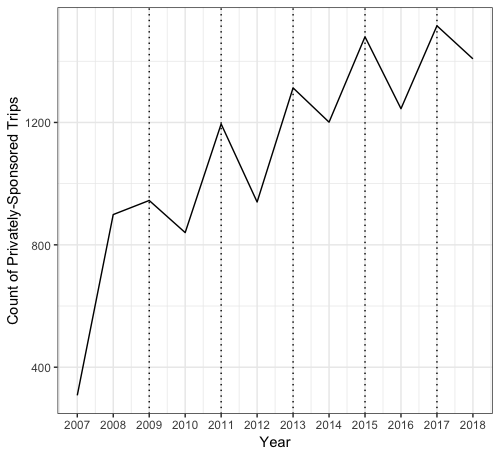
\includegraphics[scale=.55]{trend.png}
  \caption{Gift Travel by Year}
\end{figure}

\begin{figure}[hbt]
\centering
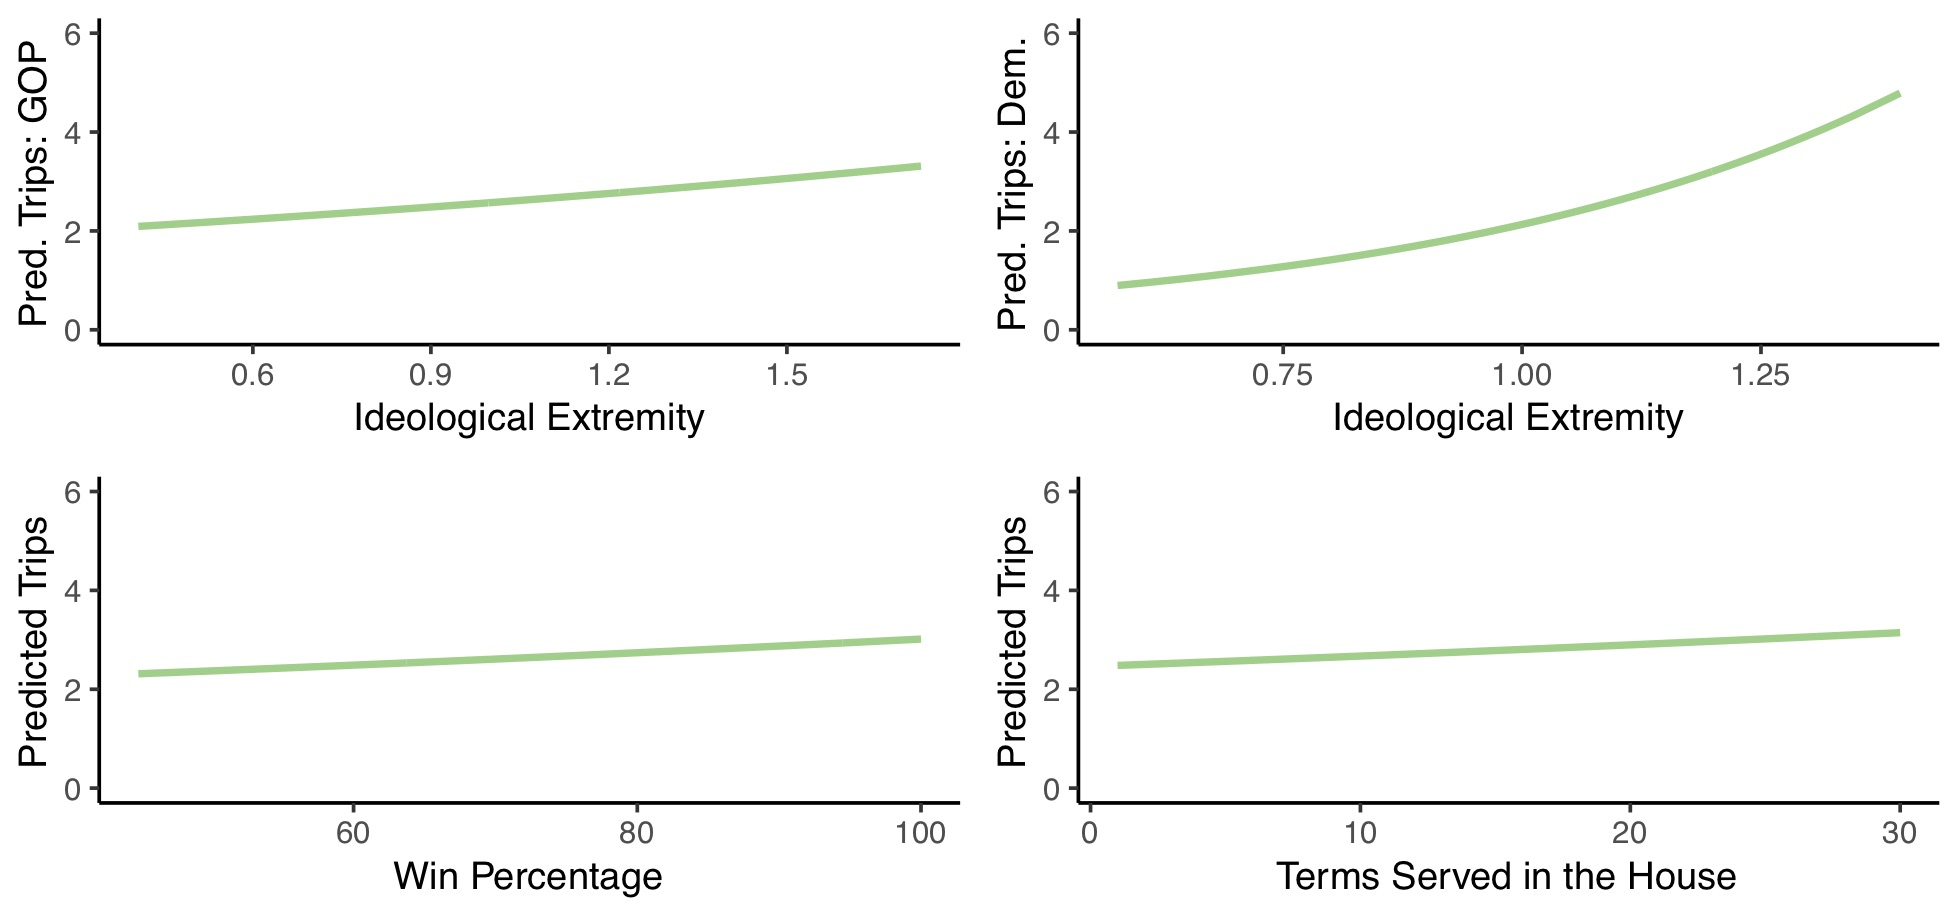
\includegraphics[scale=.21]{fig1.jpeg}
  \caption{Predicted Trips Taken by Member per Congress}
\end{figure}

\newpage
\clearpage
\setcounter{table}{0}
\renewcommand{\thetable}{A\arabic{table}}
\setcounter{page}{1}
\section*{\centering Appendix}

Appendix tables and figures? The \LaTeX code above the section header should auto-name the tables and figures as A1, A2, etc.

\end{document}
